\documentclass[a4j]{jarticle}
    \usepackage[dvipdfmx]{graphicx}
    \usepackage[ top=25truemm,bottom=37truemm,left=25truemm,right=25truemm]
    {geometry}
    \usepackage{ascmac}
    \usepackage{amsmath}
    \usepackage{array}
    \usepackage{here}
    \usepackage{url}
    \usepackage{listings, jlisting}
    \usepackage{cases}
    \usepackage{txfonts}
    \usepackage[subrefformat=parens]{subcaption}
    \renewcommand{\lstlistingname}{リスト}
\lstset{language=Python,
  basicstyle=\ttfamily\scriptsize,
  commentstyle=\textit,
  classoffset=1,
  keywordstyle=\bfseries,
  frame=tRBl,
  framesep=5pt,
  showstringspaces=false,
  numbers=left,
  stepnumber=1,
  numberstyle=\tiny,
  tabsize=4
}

\makeatletter
\def\@thesis{colabの使い方}
\def\id#1{\def\@id{#1}}
\def\department#1{\def\@department{#1}}

\def\@maketitle{
\begin{center}
{\huge \@thesis \par} %修士論文と記載される部分
\vspace{10mm}
{\LARGE\bf \@title \par}% 論文のタイトル部分
\vspace{10mm}
{\Large \@date\par}	% 提出年月日部分
\vspace{20mm}
{\Large \@department \par}	% 所属部分
{\Large  \@id \par}	% 学籍番号部分
\vspace{10mm}
{\Large  \@author}% 氏名 
\end{center}
\par\vskip 1.5em
}

\title{version1.0}
\date{更新日 2021年2月9日}
\department{}
\id{}
\author{金澤雄大}

    \begin{document}
    \maketitle
    \thispagestyle{empty}
    \clearpage
    \addtocounter{page}{-1}

    \section{Overview}
    「Google Colaboratory」でJupyter Notebookが扱えるようになりました.これによって,AnacondaをインストールしなくてもMatplotlibを使えます.
    めんどくさい環境構築とおさらばです!
    
    \section{使い方}

    まずは「Google Colaboratory」(以下colab)にアクセスしましょう.リンクは「\url{https://colab.research.google.com/notebooks/intro.ipynb}」です.
    このリンクにアクセスすると図\ref{colab-title}の画面が表示されます.プロジェクトの作成は左上の「ファイル $>$ ノートブックを新規作成」で行います.
    作成したノートブックはGoogle Driveの「Colab Notebooks」に保存されます.ノートブックで扱うCSVファイルもGoogle Driveに設置しましょう.

    \begin{figure}[H]
      \centering
      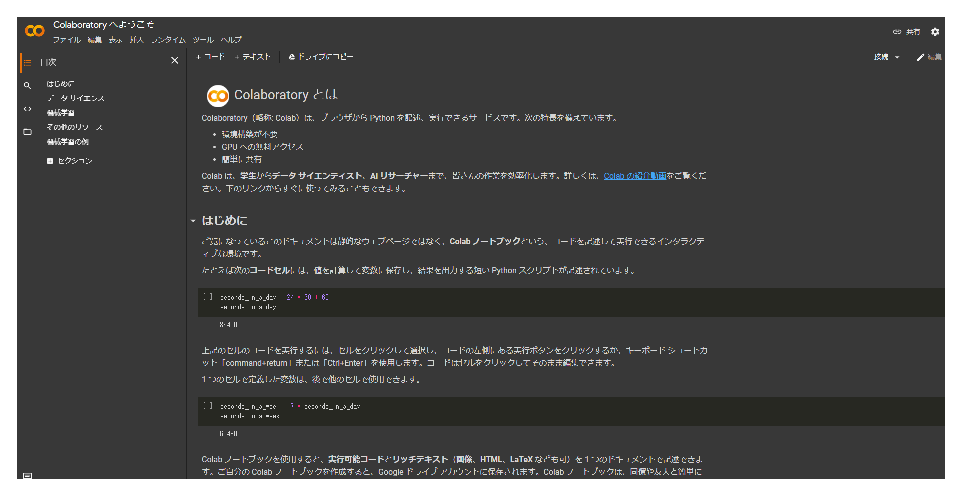
\includegraphics[scale=1.0]{colab-title.eps}
      \caption{colabへようこそ}
       \label{colab-title}
      \end{figure}

      Google Driveからファイルを読み込むためにマウントと呼ばれる作業を行います.まず,リスト\ref{mount}のコードを貼り付けて実行(Shift + Enter)
      します.リスト\ref{mount}のコードを実行すると図\ref{colab-mount1}のようになります.次に,実行結果のリンクをクリックして認証を行います.
      実行結果のリンクをクリックしてGoogleアカウントでログインしましょう.ログインすると図\ref{colab-mount2}のように連携用のコードが表示されます.
      これをコピーして,図\ref{colab-mount1}の「Enter yout authorization code :」のところに貼り付けてEnterキーを押しましょう.図\ref{colab-mount3}
      に示すように「Mounted at /content/drive」と表示されれば認証成功です.

      \begin{lstlisting}[basicstyle=\ttfamily\footnotesize, frame=single,label=mount,caption=マウントのためのコード]
from google.colab import drive
drive.mount('/content/drive')
      \end{lstlisting}

    \begin{figure}[H]
      \centering
      
\includegraphics[scale=2.0]{colab-mount.eps}
      \caption{マウントの実行1}
       \label{colab-mount1}
      \end{figure}

    \begin{figure}[H]
      \centering
      
\includegraphics[scale=2.0]{colab-code.eps}
      \caption{マウントの実行2}
       \label{colab-mount2}
      \end{figure}

    \begin{figure}[H]
      \centering
      
\includegraphics[scale=2.0]{colab-auth.eps}
      \caption{マウントの実行3}
       \label{colab-mount3}
      \end{figure}

      マウントが完了したので,データを読み込んでみましょう.ここでは,リスト\ref{testcsv}に示すtest.csvを読み込んでみます.
      test.csvをGoogle Driveに「Colab-test」というフォルダを作成して,その中に設置しました.
      \begin{lstlisting}[basicstyle=\ttfamily\footnotesize, frame=single,label=testcsv,caption=test.csv]
1,5
2,11
3,14
4,22
5,28
      \end{lstlisting}

      読み込みはリスト\ref{read}のプログラムで行います.リスト\ref{read}の2行目がデータを読み込むためのコードです.
      「/content/drive/My Drive/」以下はディレクトリの構造によって逐次変更してください.図\ref{colab-result1}のように
      表形式で読み込んだCSVファイルの中身が表示されれば成功です.
      \begin{lstlisting}[basicstyle=\ttfamily\footnotesize, frame=single,label=read,caption=データの読み込み]
import pandas as pd
df = pd.read_csv("/content/drive/My Drive/Colab-data/test.csv",header=None)
df.head()
      \end{lstlisting}

      \begin{figure}[H]
        \centering
        
\includegraphics[scale=2.0]{colab-result1.eps}
        \caption{CSV読み込みの実行結果}
         \label{colab-result1}
        \end{figure}

        colabのmatplotlibで日本語を使うためには,リスト\ref{jp}のように「japanize\_matplotlib」を読み込む必要があります.
        リスト\ref{jp}を実行して図\ref{colab-result2}のようになれば成功です.
        \begin{lstlisting}[basicstyle=\ttfamily\footnotesize, frame=single,label=jp,caption=日本語対応のコード]
!pip install japanize-matplotlib
import matplotlib.pyplot as plt
import japanize_matplotlib 

plt.figure(facecolor="white")
plt.plot(df[0],df[1])
plt.xlabel("x")
plt.xlabel("y")
plt.title("日本語対応テスト")          
        \end{lstlisting}

        \begin{figure}[H]
          \centering
          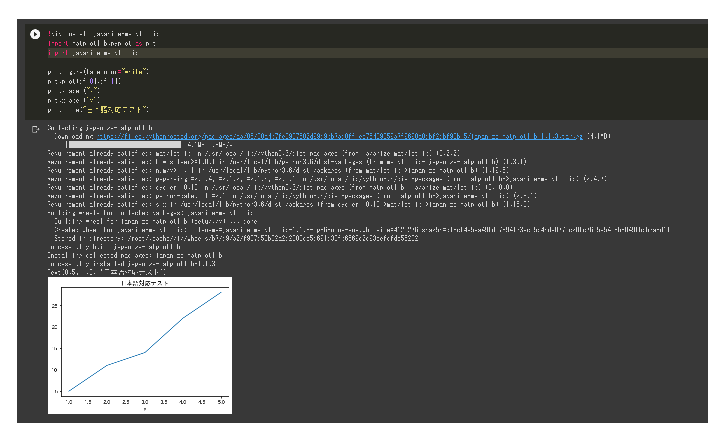
\includegraphics[scale=1.3]{colab-result2.eps}
          \caption{colabの日本語対応}
           \label{colab-result2}
          \end{figure}

\end{document}

